
% Papel A4, fonte Times tamanho 12
\documentclass[a4paper,12pt]{article}
% Determinando tamanhos de margens
\usepackage[left=2cm, right=2cm, top=3cm, bottom=1cm]{geometry}
% Preâmbulo para documentos em português
\usepackage[brazilian]{babel}
\usepackage[utf8]{inputenc}
\usepackage[T1]{fontenc}
\usepackage[pdftex]{graphicx}
\usepackage{color}
\usepackage{fancyhdr}
\usepackage{multirow}
\usepackage{hhline}
\usepackage[skip=0pt]{caption}

\begin{document}

\pagestyle{fancy}
\fancyhead[R]{
\includegraphics[width = 4cm]{logo_simepar.png}}
\renewcommand{\headrulewidth}{1pt}
\begin{center}
\vspace{10pt}
\Large{\textbf{Previsão de Afluência - Reservatório de Fiu}}\\
\Large{\textbf{2021-03-10}}
\noindent
\rule{\textwidth}{1pt}
\end{center}

\vspace{6pt}
\textbf{\large{Localização das estações}}

\begin{figure}[ht]
    \centering
    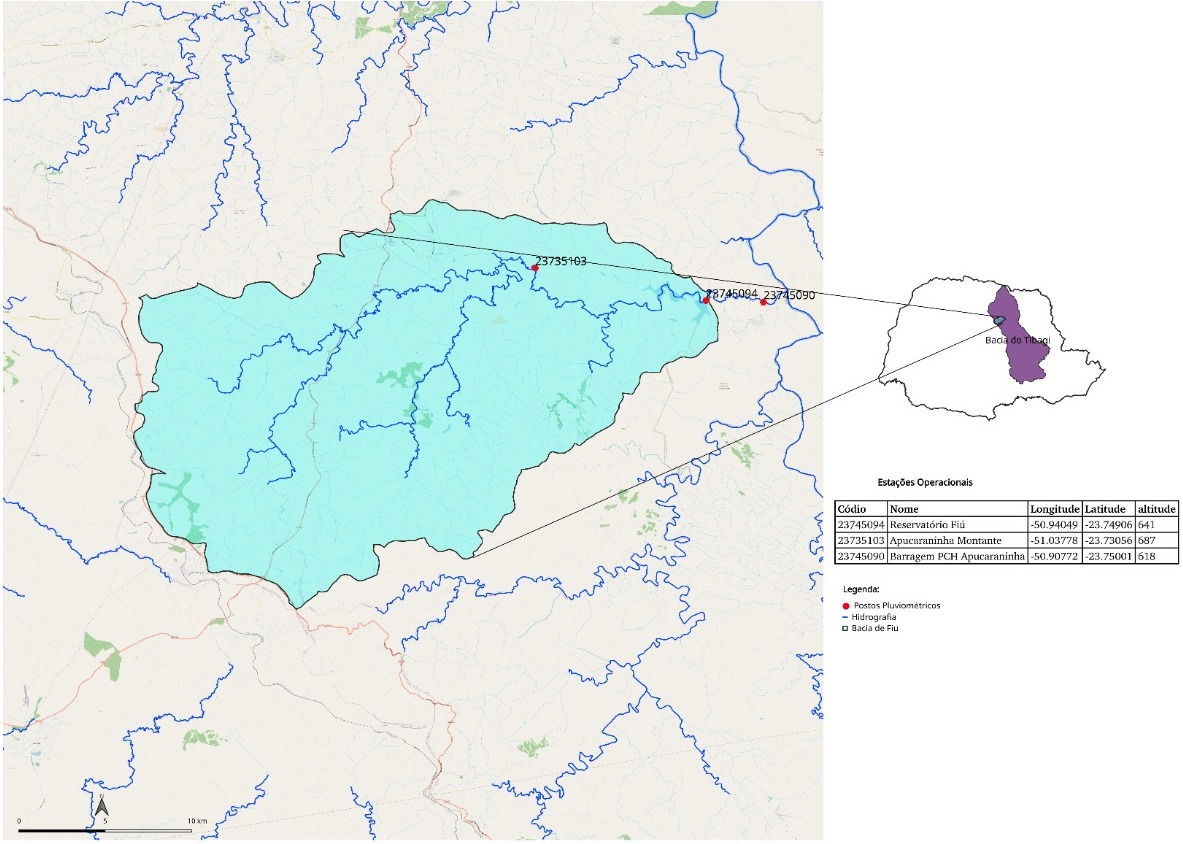
\includegraphics[height=300pt]{area_fiu.jpeg}
    \vspace{6pt}
    \caption{Bacia de Fiu}
\end{figure}

\vspace{6pt}
\textbf{\large{Chuva Observada}}

\begin{table}[ht]
    \centering
    \caption{Dados de chuva observada na bacia}
    \vspace{6pt}
    \begin{tabular}{|c|c|c|c|c|}
        \hline
        & \multicolumn{3}{|c|}{Estação} & \\
        \hhline{~---~}
        & Apucaraninha & Barragem PCH & & \\
        & Montante & Apucaraninha & Reservatório Fiu & Chuva Integrada \\
        \hhline{~----}
        Dia & \multicolumn{4}{|c|}{Precipitação (mm)} \\
        \hline
        2021-03-03 & 5.8 & 3.8 & 4.6 & 7.8 \\
        \hline
        2021-03-04 & 9.4 & 1.0 & 1.6 & 7.5 \\
        \hline
        2021-03-05 & 9.0 & 9.8 & 10.6 & 13.8 \\
        \hline
        2021-03-06 & 0.2 & 20.4 & 34.6 & 8.0 \\
        \hline
        2021-03-07 & 3.2 & 10.2 & 15.0 & 5.7 \\
        \hline
        2021-03-08 & 1.0 & 0.2 & 0.2 & 0.2 \\
        \hline
        2021-03-09 & 5.2 & 2.4 & 7.2 & 3.7 \\
        \hline
    \end{tabular}
\end{table}

\newpage
\textbf{\large{Previsão Hidrometeorológica}}
\smallbreak
\textbf{\small{Modelo Sacramento}}\\
\begin{figure}[ht]
    \centering
    \vspace{-24pt}
    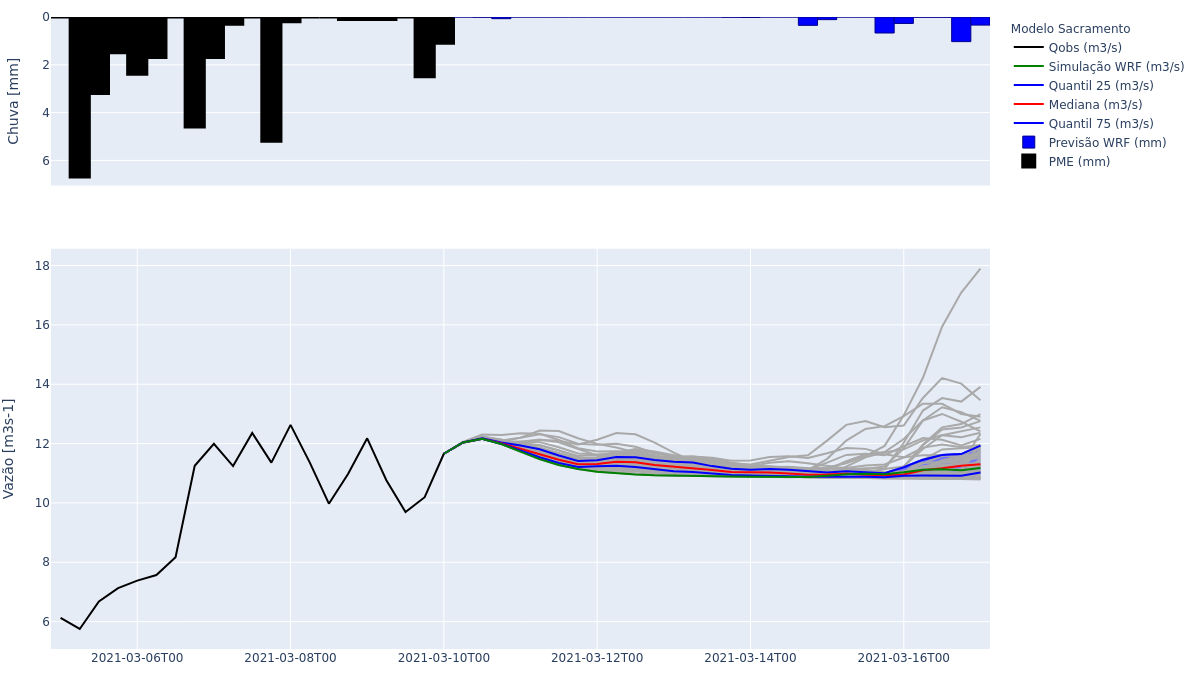
\includegraphics[width=\textwidth]{fig_sac_2021031000.png}
    \caption{Previsão de afluência para o reservatório - Modelo Sacramento}
\end{figure}

\textbf{\small{Modelo GR5i}}\\
\begin{figure}[ht]
    \centering
    \vspace{-24pt}
    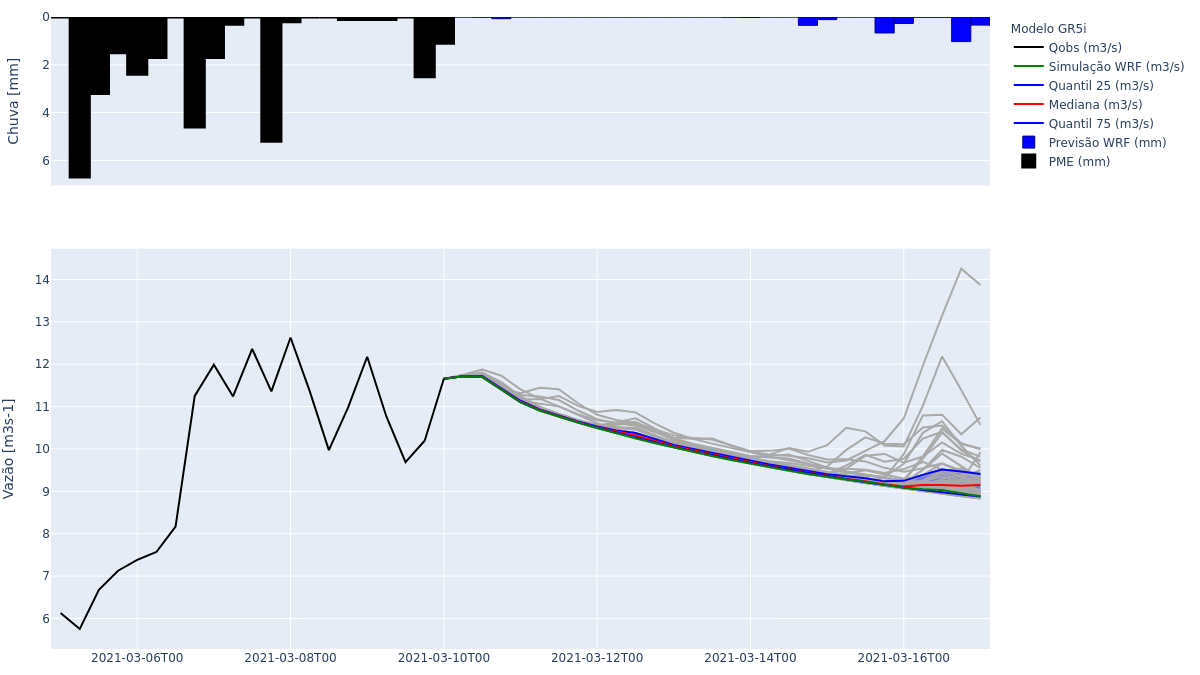
\includegraphics[width=\textwidth]{fig_gr5i_2021031000.png}
    \caption{Previsão de afluência para o reservatório - Modelo GR5i}
\end{figure}

\newpage
\textbf{\large{Detalhamento Previsões}}
\begin{table}[ht]
    \centering
    \caption{Valores de vazão afluente média prevista - Modelo Sacramento}
    \vspace{6pt}
    \begin{tabular}{|c|c|c|c|c|c|c|}
        \hline
        & \multicolumn{5}{|c|}{Simulação com chuva ECMWF} & Simulação com \\
        \hhline{~-----~}
        & Mínimo & Quantil 25 & Mediana & Quantil 75 & Máximo & chuva WRF \\
        \hhline{~------}
        Hora & \multicolumn{6}{|c|}{Vazão Média Prevista (m3s-1)} \\
        \hline
        2021-03-10T00 & 11.657 & 11.657 & 11.657 & 11.657 & 11.657 & 11.657 \\
        \hline
        2021-03-10T06 & 12.038 & 12.038 & 12.039000000000001 & 12.04 & 12.059000000000001 & 12.038 \\
        \hline
        2021-03-10T12 & 12.159 & 12.161 & 12.164000000000001 & 12.174000000000001 & 12.302 & 12.16 \\
        \hline
        2021-03-10T18 & 11.985 & 11.994000000000002 & 12.008 & 12.036 & 12.289000000000001 & 11.987 \\
        \hline
        2021-03-11T00 & 11.727 & 11.769 & 11.827 & 11.937000000000001 & 12.345 & 11.728 \\
        \hline
        2021-03-11T06 & 11.474 & 11.540999999999999 & 11.648 & 11.809000000000001 & 12.439 & 11.477 \\
        \hline
        2021-03-11T12 & 11.275 & 11.347999999999999 & 11.452 & 11.6 & 12.422 & 11.279000000000002 \\
        \hline
        2021-03-11T18 & 11.140999999999998 & 11.210999999999999 & 11.306 & 11.41 & 12.179 & 11.14 \\
        \hline
        2021-03-12T00 & 11.050999999999998 & 11.237 & 11.315 & 11.440999999999999 & 12.129000000000001 & 11.049000000000001 \\
        \hline
        2021-03-12T06 & 11.002 & 11.255 & 11.384 & 11.548 & 12.353 & 10.993 \\
        \hline
        2021-03-12T12 & 10.968 & 11.214 & 11.370999999999999 & 11.540999999999999 & 12.311 & 10.958 \\
        \hline
        2021-03-12T18 & 10.936 & 11.132 & 11.275 & 11.448 & 12.032 & 10.93 \\
        \hline
        2021-03-13T00 & 10.919 & 11.065 & 11.222999999999999 & 11.385 & 11.695 & 10.915 \\
        \hline
        2021-03-13T06 & 10.908 & 11.038 & 11.175 & 11.36 & 11.564 & 10.905999999999999 \\
        \hline
        2021-03-13T12 & 10.899000000000001 & 10.979000000000001 & 11.107000000000001 & 11.24 & 11.522 & 10.898 \\
        \hline
        2021-03-13T18 & 10.890999999999998 & 10.944 & 11.045 & 11.148 & 11.418 & 10.89 \\
        \hline
        2021-03-14T00 & 10.883 & 10.922 & 11.04 & 11.116 & 11.431 & 10.884 \\
        \hline
        2021-03-14T06 & 10.875 & 10.921 & 11.023 & 11.142000000000001 & 11.547 & 10.880999999999998 \\
        \hline
        2021-03-14T12 & 10.867 & 10.897 & 10.991 & 11.114 & 11.575 & 10.876 \\
        \hline
        2021-03-14T18 & 10.859000000000002 & 10.88 & 10.948 & 11.068 & 11.607000000000001 & 10.877 \\
        \hline
        2021-03-15T00 & 10.850999999999999 & 10.887 & 10.953 & 11.027999999999999 & 12.1 & 10.92 \\
        \hline
        2021-03-15T06 & 10.844000000000001 & 10.895999999999999 & 10.979000000000001 & 11.069 & 12.63 & 10.97 \\
        \hline
        2021-03-15T12 & 10.835999999999999 & 10.880999999999998 & 10.949000000000002 & 11.044 & 12.757 & 10.98 \\
        \hline
        2021-03-15T18 & 10.829 & 10.865 & 10.93 & 11.002 & 12.587 & 10.97 \\
        \hline
        2021-03-16T00 & 10.821 & 10.913 & 10.959000000000001 & 11.200999999999999 & 12.950999999999999 & 11.030999999999999 \\
        \hline
        2021-03-16T06 & 10.814 & 10.921 & 11.097999999999999 & 11.455 & 14.218 & 11.115 \\
        \hline
        2021-03-16T12 & 10.806 & 10.922 & 11.169 & 11.617 & 15.939 & 11.130999999999998 \\
        \hline
        2021-03-16T18 & 10.799000000000001 & 10.914000000000001 & 11.255 & 11.645 & 17.088 & 11.103 \\
        \hline
        2021-03-17T00 & 10.793 & 11.022 & 11.300999999999998 & 11.929 & 17.891 & 11.175999999999998 \\
        \hline
    \end{tabular}
    \vspace{-12pt}
\end{table}

\begin{itemize}
    \item Horário de disparo da previsão: 2021-03-04T00:00 (UTC).
    \item Horários registrados pelo Tempo Coordenado Universal (UTC) / Hora Mundial.
    \item Dados indexados no limite superior de tempo. Ex: Registro de 06:00 contém previsões de vazão média para período 00:01 a 06:00.
    \item Simulações com Ensemble ECMWF - Conjunto de 51 forçantes.
\end{itemize}

\newpage
\begin{table}[ht]
    \centering
    \caption{Valores de vazão afluente média prevista - Modelo GR5i}
    \vspace{6pt}
    \begin{tabular}{|c|c|c|c|c|c|c|}
        \hline
        2021-03-10T00 & 11.657 & 11.657 & 11.657 & 11.657 & 11.657 & 11.657 \\
        \hline
        2021-03-10T06 & 11.715 & 11.716 & 11.716 & 11.719000000000001 & 11.75 & 11.715 \\
        \hline
        2021-03-10T12 & 11.702 & 11.704 & 11.708 & 11.72 & 11.875 & 11.702 \\
        \hline
        2021-03-10T18 & 11.392999999999999 & 11.397 & 11.405 & 11.427999999999999 & 11.729000000000001 & 11.392999999999999 \\
        \hline
        2021-03-11T00 & 11.104000000000001 & 11.107000000000001 & 11.116 & 11.137 & 11.405999999999999 & 11.104000000000001 \\
        \hline
        2021-03-11T06 & 10.908 & 10.91 & 10.92 & 10.934000000000001 & 11.443 & 10.908 \\
        \hline
        2021-03-11T12 & 10.763 & 10.765 & 10.772 & 10.790999999999999 & 11.41 & 10.763 \\
        \hline
        2021-03-11T18 & 10.626 & 10.628 & 10.635 & 10.651 & 11.078 & 10.626 \\
        \hline
        2021-03-12T00 & 10.495 & 10.502 & 10.51 & 10.533 & 10.874 & 10.495 \\
        \hline
        2021-03-12T06 & 10.37 & 10.384 & 10.412 & 10.439 & 10.917 & 10.37 \\
        \hline
        2021-03-12T12 & 10.252 & 10.277000000000001 & 10.319 & 10.378 & 10.864 & 10.252 \\
        \hline
        2021-03-12T18 & 10.14 & 10.158999999999999 & 10.193999999999999 & 10.235 & 10.606 & 10.14 \\
        \hline
        2021-03-13T00 & 10.033 & 10.046 & 10.071 & 10.095 & 10.384 & 10.033 \\
        \hline
        2021-03-13T06 & 9.93 & 9.948 & 9.969 & 10.001 & 10.259 & 9.93 \\
        \hline
        2021-03-13T12 & 9.833 & 9.852 & 9.872 & 9.91 & 10.247 & 9.833 \\
        \hline
        2021-03-13T18 & 9.74 & 9.758 & 9.776 & 9.808 & 10.084 & 9.74 \\
        \hline
        2021-03-14T00 & 9.65 & 9.667 & 9.685 & 9.715 & 9.949 & 9.651 \\
        \hline
        2021-03-14T06 & 9.564 & 9.584 & 9.599 & 9.635 & 9.955 & 9.568 \\
        \hline
        2021-03-14T12 & 9.482999999999999 & 9.505 & 9.521 & 9.557 & 10.02 & 9.488999999999999 \\
        \hline
        2021-03-14T18 & 9.405 & 9.425 & 9.442 & 9.472000000000001 & 9.933 & 9.408999999999999 \\
        \hline
        2021-03-15T00 & 9.333 & 9.35 & 9.367 & 9.402999999999999 & 10.091000000000001 & 9.336 \\
        \hline
        2021-03-15T06 & 9.263 & 9.283 & 9.297 & 9.357000000000001 & 10.499 & 9.277000000000001 \\
        \hline
        2021-03-15T12 & 9.193999999999999 & 9.215 & 9.24 & 9.308 & 10.415999999999999 & 9.225 \\
        \hline
        2021-03-15T18 & 9.128 & 9.147 & 9.166 & 9.236 & 10.183 & 9.149 \\
        \hline
        2021-03-16T00 & 9.062999999999999 & 9.09 & 9.116 & 9.247 & 10.72 & 9.082 \\
        \hline
        2021-03-16T06 & 9.002 & 9.032 & 9.149 & 9.389 & 11.97 & 9.052 \\
        \hline
        2021-03-16T12 & 8.943 & 8.972000000000001 & 9.152000000000001 & 9.513 & 13.145 & 9.033999999999999 \\
        \hline
        2021-03-16T18 & 8.885 & 8.927 & 9.131 & 9.466000000000001 & 14.253 & 8.954 \\
        \hline
        2021-03-17T00 & 8.83 & 8.88 & 9.151 & 9.408999999999999 & 13.870999999999999 & 8.882 \\
        \hline
    \end{tabular}
    \vspace{-12pt}
\end{table}

\begin{itemize}
    \item Horário de disparo da previsão: 2021-03-04T00:00 (UTC).
    \item Horários registrados pelo Tempo Coordenado Universal (UTC) / Hora Mundial.
    \item Dados indexados no limite superior de tempo. Ex: Registro de 06:00 contém previsões de vazão média para período 00:01 a 06:00.
    \item Simulações com Ensemble ECMWF - Conjunto de 51 forçantes.
\end{itemize}

\end{document}
